\documentclass[11pt]{article}

%% MinionPro fonts 
%\usepackage[lf]{MinionPro}
%\usepackage{MnSymbol}
\usepackage{microtype}

%% Margins
\usepackage{geometry}
\geometry{verbose,letterpaper,tmargin=1in,bmargin=1in,lmargin=1in,rmargin=1in}

%% Other packages
\usepackage{amsmath}
\usepackage{amsthm}
\usepackage[shortlabels]{enumitem}
\usepackage{titlesec}
\usepackage{soul}
\usepackage{tikz}
\usepackage{mathtools}
\usepackage{pgfplots}
\usepackage{tikz-3dplot}
\usepackage{algorithmic}
\usepackage[export]{adjustbox}
\usepackage{tcolorbox}
\usepackage{xcolor}
\newcommand{\blu}{\color{blue}}
%% Paragraph style settings
\setlength{\parskip}{\medskipamount}
\setlength{\parindent}{0pt}

%% Change itemize bullets
\renewcommand{\labelitemi}{$\bullet$}
\renewcommand{\labelitemii}{$\circ$}
\renewcommand{\labelitemiii}{$\diamond$}
\renewcommand{\labelitemiv}{$\cdot$}

%% Colors
\definecolor{rred}{RGB}{204,0,0}
\definecolor{ggreen}{RGB}{0,145,0}
\definecolor{yyellow}{RGB}{255,185,0}
\definecolor{bblue}{rgb}{0.2,0.2,0.7}
\definecolor{ggray}{RGB}{190,190,190}
\definecolor{ppurple}{RGB}{160,32,240}
\definecolor{oorange}{RGB}{255,165,0}

%% Shrink section fonts
\titleformat*{\section}{\normalsize\bf}
\titleformat*{\subsection}{\normalsize\bf}
\titleformat*{\subsubsection}{\normalsize\it}

% %% Compress the spacing around section titles
\titlespacing*{\section}{0pt}{1.5ex}{0.75ex}
\titlespacing*{\subsection}{0pt}{1ex}{0.5ex}
\titlespacing*{\subsubsection}{0pt}{1ex}{0.5ex}

%% amsthm settings
\theoremstyle{definition}
\newtheorem{problem}{Problem}
\newtheorem{example}{Example}
\newtheorem*{theorem}{Theorem}
\newtheorem*{bigthm}{Big Theorem}
\newtheorem*{biggerthm}{Bigger Theorem}
\newtheorem*{bigcor1}{Big Corollary 1}
\newtheorem*{bigcor2}{Big Corollary 2}

%% tikz settings
\usetikzlibrary{calc}
\usetikzlibrary{patterns}
\usetikzlibrary{decorations}
\usepgfplotslibrary{polar}

%% algorithmic setup
\algsetup{linenodelimiter=}
\renewcommand{\algorithmiccomment}[1]{\quad// #1}
\renewcommand{\algorithmicrequire}{\emph{Input:}}
\renewcommand{\algorithmicensure}{\emph{Output:}}

%% Answer box macros
%% \answerbox{alignment}{width}{height}
\newcommand{\answerbox}[3]{%
  \fbox{%
    \begin{minipage}[#1]{#2}
      \hfill\vspace{#3}
    \end{minipage}
  }
}

%% \answerboxfull{alignment}{height}
\newcommand{\answerboxfull}[2]{%
  \answerbox{#1}{6.38in}{#2} 
}

%% \answerboxone{alignment}{height} -- for first-level bullet
\newcommand{\answerboxone}[2]{%
  \answerbox{#1}{6.0in}{#2} 
}

%% \answerboxtwo{alignment}{height} -- for second-level bullet
\newcommand{\answerboxtwo}[2]{%
  \answerbox{#1}{5.8in}{#2}
}

%% special boxes
\newcommand{\wordbox}{\answerbox{c}{1.2in}{.5cm}}
\newcommand{\catbox}{\answerbox{c}{.5in}{.7cm}}
\newcommand{\letterbox}{\answerbox{c}{.7cm}{.5cm}}

%% Miscellaneous macros
\newcommand{\tstack}[1]{\begin{multlined}[t] #1 \end{multlined}}
\newcommand{\cstack}[1]{\begin{multlined}[c] #1 \end{multlined}}
\newcommand{\ccite}[1]{\only<presentation>{{\scriptsize\color{gray} #1}}\only<article>{{\small [#1]}}}
\newcommand{\grad}{\nabla}
\newcommand{\ra}{\ensuremath{\rightarrow}~}
\newcommand{\maximize}{\text{maximize}}
\newcommand{\minimize}{\text{minimize}}
\newcommand{\subjectto}{\text{subject to}}
\newcommand{\trans}{\mathsf{T}}
\newcommand{\bb}{\mathbf{b}}
\newcommand{\bx}{\mathbf{x}}
\newcommand{\bc}{\mathbf{c}}
\newcommand{\bd}{\mathbf{d}}

%% LP format
%    \begin{align*}
%      \maximize \quad & \mathbf{c}^{\trans} \mathbf{x}\\
%      \subjectto \quad & A \mathbf{x} = \mathbf{b}\\
%                       & \mathbf{x} \ge \mathbf{0}
%    \end{align*}


%% Redefine maketitle
\makeatletter
\renewcommand{\maketitle}{
  \noindent SA405 -- AMP \hfill \\

  \begin{center}\Large{\textbf{\@title}}\end{center}
}
\makeatother

%% ----- Begin document ----- %%
\begin{document}
  
\title{MiniProject 2:  Vehicle Routing Problem}

\maketitle

{\blu \Large \textbf{IP Model and Python Implementation}}
	\begin{itemize}
	\item Formulation and python implementation due \textbf{Tuesday 2 November at 2359}
	\end{itemize}

{\blu \Large \bf Ground Rules:}
	\begin{itemize}
	\item This is an individual project
	\item You may ask me for help, your textbook/notes, or Google but cite your sources.
	\end{itemize}

%%%
\section{The Problem}

The USNA coffee company has decided to start delivering (iced) coffee around the yard. The diagram below shows the location of the coffee company (location 0) and the coordinates of each customer on the yard. Assume that each customer has the same demand. The USNA coffee company has four (4) people who are available to deliver coffee and each of which can deliver to up to five customers.  Distances are the direct, straight-line, distance between points.

\begin{center}
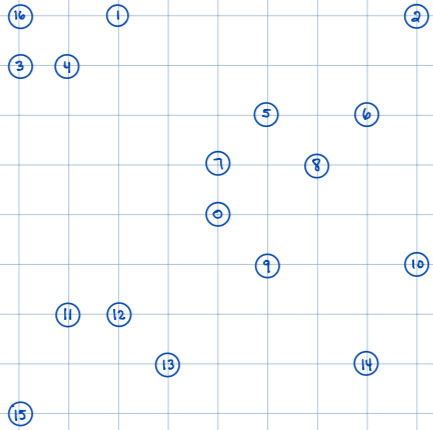
\includegraphics[width=0.7\textwidth]{map.png}
\end{center}

\newpage

\noindent{\Large \textbf{Part 1: Formulation.}} Formulate this model as a vehicle routing problem.
	\begin{enumerate}[a.]
	\item Write a concrete model for this VRP model. Do \textbf{not} include subtour elimination constraints.
	\item Convert your model to a parameterized VRP model with generalized subtour elimination constraints.
	\end{enumerate}

\vspace{0.5in}

%\section{The Assignment}
\noindent{\Large \textbf{Part 2:  Python implementation with manual subtour elimination constraints.}}
\begin{enumerate}[a.]
\item Using the project 2 starter file, complete the Jupyter notebook to implement your VRP model.
\item For iteratively adding subtour elimination constraints, at each step, explain why your current solution is wrong and what you need to change before you solve the problem again.
\item To make sure you're on the right track, your initial solution, with no subtour elimination constraints, will have an objective function value of \verb|44.59856358193051|
\end{enumerate}

\vspace{0.5in}

\noindent{\Large \textbf{Grading: }} For grading, submit both your formulation and Jupyter notebook. The formulation will count as 25\% of your project 2 grade while the python code will count for 75\% of your project 2 grade.

\vspace{0.5in}

\noindent{\Large \textbf{OPTIONAL BONUS: }} In modern solvers for VRP/TSP, the subtour elimination constraints are automated. As an optional bonus, modify your Jupyter notebook to automate the cycle elimination constraints. That is, if I run your notebook, I run it once and it will produce the final solution while eliminating cycles as it goes without user input. To do so, you need to determine how to detect a cycle based on a given solution and how to automate the cycle elimination constraints. This is completely \textbf{optional}, but if you do it correctly bonus points will be added to your project 2 grade.

Hint for the bonus: In order to automate adding constraints, you need to add multiple constraints of similar names. One easy way to do this is to use the function \verb|model.add_component|. For example, if I want to add my favorite constraint iteratively, one way to do it is:

\verb|model.add_component(f'my_const_{counter}',pyo.Constraint(rule=my_const_rule))|

Where counter is the index of the constraint I'd like to add.

\end{document}
